

%-----------------------------------------------------------------------------%
\chapter{\babSatu}

%-----------------------------------------------------------------------------%
%-----------------------------------------------------------------------------%


\section{Latar Belakang}

%-----------------------------------------------------------------------------%
Bahasa merupakan representasi perilaku kompleks yang dimiliki oleh spesies dengan tingkat kognisi tinggi. Elemen suara, kata-kata, dan pola sintaktis sebuah bahasa berbeda untuk setiap kelompok manusia dan berkembang secara perlahan menjadi bentuk bahasa yang paling efisien \citep{aitchison_2004}. Hal ini disebabkan oleh berkembangnya pola linguistik seiring waktu dan penyebaran \citep{sapir_1921}. \cite{chomsky_1965} juga mengungkapkan bahwa keserupaan dari semua bahasa di dunia adalah aspek kreatifnya, sehingga memungkinkan penutur untuk mengekspresikan pikiran dengan jumlah yang tak terhingga dan bereaksi secara tepat dalam segala bentuk situasi. Salah satu karakteristik ujaran manusia yang paling utama adalah tingkat keteraturan atau organisasi isi tuturan yang sangat tinggi. Semua satuan yang membentuk sebuah tuturan disusun oleh penutur dengan konfigurasi yang sangat spesifik mengikuti aturan tertentu. Aturan-aturan ini membentuk tataran organisasi terpenting dari sebuah bahasa, yaitu sintaksis. Para linguis Jerman terdahulu menerjemahkan kata sintaksis ke dalam bahasa Jerman sebagai \textit{Satzlehre} atau 'ilmu kalimat' karena obyek dari sintaksis struktural adalah studi tentang kalimat \citep{tesniere_1959}.

Dalam kajian-kajian linguistik transformasional, para linguis memisahkan antara pengetahuan penutur terhadap sebuah bahasa untuk dapat memproduksi dan memahami bahasanya dengan bagaimana penutur menggunakan pengetahuan tersebut secara nyata untuk berbicara, memahami, membaca, dan menulis (\citealp{chomsky_1965,delahunty_garvey_2010}). Manusia memiliki kemampuan mental dan kognisi untuk mempelajari, memproduksi, dan mengerti ujaran yang berbeda-beda. Pengetahuan bawah sadar terhadap aturan yang membentuk sebuah bahasa ini disebut dengan kompetensi (\textit{competence}). Sementara itu, aktivitas linguistik yang memanfaatkan pengetahuan tersebut secara nyata disebut dengan performa (\textit{performance}). \cite{chomsky_1965} menekankan bahwa investigasi terhadap \textit{performance} hanya akan bermakna sejauh pemahaman terhadap \textit{competence} yang mendasarinya.

Beberapa linguis lain seperti \cite{sag_wasow_2011} berargumen dan mengungkapkan pentingnya penelitian mengenai \textit{performance} yang dapat menjadi basis fakta empiris dalam perkembangan teori-teori gramatikal atau \textit{competence}. \cite{hawkins_2014} juga mengeksplorasi keterkaitan antara \textit{performance} dan konvensi tata bahasa dan mengungkapkan bahwa kecenderungan yang ditemukan dalam data penggunaan bahasa yang mencakup pilihan penutur (urutan kata, pilihan klausa, dan lain-lain) tampak serupa dengan kecenderungan yang ditemukan dalam konvensi tata bahasa. Hawkins berasumsi bahwa aturan tata bahasa sudah merefleksikan keterbatasan memori serta bentuk efisiensi dan kompleksitas lain yang diobservasi dalam data penggunaan bahasa atau \textit{performance}. Namun, asumsi ini baru memiliki bukti kuat dalam penelitian terhadap bahasa-bahasa dengan urutan kata yang lebih pasti (\textit{fixed word order}). 

Berbagai penelitian lintas bahasa telah dilakukan untuk menunjukkan bahwa banyak bahasa di dunia tidak terkekang oleh struktur urutan kata sesederhana Subyek, Predikat, dan Obyek seperti dalam Bahasa Inggris yang urutan Subyek dan Predikat-nya bisa berubah (\citealp{macwhinney_bates_1989, birner_ward_1998, lambrecht_2000}). Perbedaan urutan kata dapat dimotivasi oleh bebagai aspek seperti kala waktu, kepastian, dan \textit{animacy} (\citealp{dryer1992greenbergian, tsunoda1995adpositions, polinskaja1989object}).  \cite{hawkins1994performance} berargumen bahwa terdapat keterkaitan konsep urutan kata antara bahasa-bahasa dengan \textit{free word order} dan \textit{fixed word order}, yaitu bahwa urutan kata yang banyak digunakan oleh penutur pada bahasa dengan \textit{free word order} serupa dengan urutan kata yang dikonvensionalisasikan secara aktif pada bahasa dengan \textit{fixed word order}. \cite{hawkins1994performance} mengaitkan pilihan terhadap urutan kata tertentu ke dalam asas efisiensi bahasa yang dikembangkannya dan mengatakan bahwa jenis urutan kata tertentu memudahkan pendengar memproses informasi dibandingkan yang lain.

Kesimpulan bahwa Bahasa Indonesia tergolong memiliki urutan kata yang bebas banyak muncul dalam penelitian mengenai urutan kata pada ranah sintaksis (\citealp{stack2005word, postman2004processing}). \cite{sneddon2010indonesian} mengungkapkan bahwa meskipun Bahasa Indonesia memiliki basis urutan kata tertentu, berbagai kondisi memungkinkannya untuk berubah, seperti contoh perbedaan penekanan yang mengakibatkan perbedaan urutan kata antara "Endang lari ke toko dengan cepat" dan "Dengan cepat Endang lari ke toko". Dalam penelitiannya, \cite{postman2004processing} menekankan bahwa Bahasa Indonesia merupakan bahasa yang berorientasi pada tema sehingga tidak memiliki urutan kata resmi yang jelas. Pada aspek efisiensi, John McWhorter menulis sebuah artikel di media online The Atlantic \citep{mcwhorter2016efficient} dengan memaparkan beberapa bukti ujaran dari penutur Bahasa Indonesia untuk menunjukkan bagaimana Bahasa Indonesia merupakan salah satu bahasa paling efisien dan ekonomis. McWhorter menambahkan bahwa tata bahasa dalam Bahasa Indonesia juga secara periodik diolah secara organik oleh para penuturnya sehingga terdapat keteraturan bentuk bahkan dalam bahasa sehari-hari (informal). Urutan kata dan efisiensi dalam Bahasa Indonesia ini sangat berkaitan dengan perdebatan antara hubungan \textit{competence} dan \textit{performance} di dunia linguistik, terutama dikarenakan tingginya fleksibilitas yang dimiliki oleh Bahasa Indonesia.

Selama puluhan tahun, banyak riset dilakukan untuk melihat bagaimana penutur mengatur dan memproduksi bahasa menjadi bentuk yang paling efisien (Chomsky, 2005; Hawkins, 2004; Zipf, 1935,1949). Beberapa kajian linguistik modern yang menyoroti masalah ini memanfaatkan teori dependensi. Dependensi adalah gagasan bahwa setiap unit linguistik terhubung satu sama lain oleh tautan langsung karena memiliki relasi semantik (Tesni�re, 1959). Sebagai contoh, penutur Bahasa Indonesia harus menuturkan Saya cinta kamu dan bukan *Saya kamu cinta seperti dalam bahasa Perancis (Je t?aime). Pada kedua kalimat tersebut, terlihat perbedaan bagaimana posisi subyek dan obyek bergantung pada predikatnya. Contoh kasus sederhana tersebut menunjukkan bahwa kata-kata sebagai konstituen kalimat terhubung oleh tautan langsung yang disebut juga dengan dependensi (dependency). Teori dependensi merupakan teori sintaksis modern namun memanfaatkan konsep dasar linguistik seperti halnya konsep penanda dan petanda (Saussure, 1983 [1916]). 

Menurut Saussure, untuk dapat mengantarkan informasi tertentu, penutur harus memilih tanda pada sumbu paradigmatik dan mengatur tanda tersebut ke dalam urutan linear pada sumbu sintagmatik. Dalam teori dependensi, satu kata harus bergantung kepada kata lain untuk menduduki posisi linear tertentu dan membentuk relasi sintagmatik (Tesni�re, 1959). Dengan kata lain, pengaturan tanda pada sumbu sintagmatik dikendalikan oleh dependensi yang menghubungkan konstituen-konstituen tersebut. Perbedaan dependensi tidak hanya berlaku secara lintas bahasa seperti pada contoh kasus dalam Bahasa Indonesia dan Perancis di atas, tetapi juga dapat ditemukan dalam satu bahasa seperti pada Gambar 1 sehingga dapat memberikan gambaran keterkaitan struktur konstruksi kalimat dengan kerja kognisi manusia (Gibson, 2000). Posisi kata keluar pada urutan linear kedua kalimat berbeda, sehingga jarak dependensi antara kata membuang dan keluar pada kedua kalimat juga berbeda (\pic~\ref{fig:gambar11}). 
\begin{figure}
	\centering 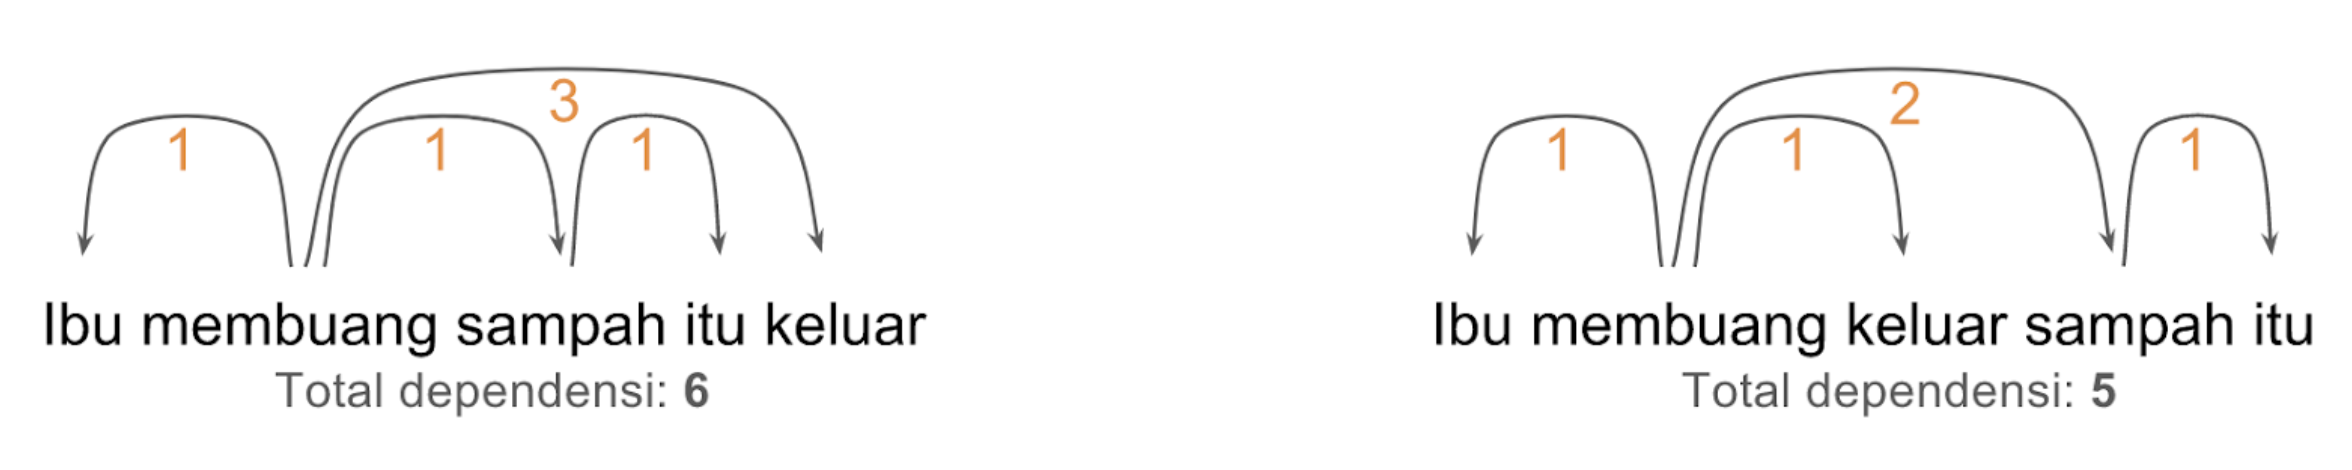
\includegraphics[width=1
	\textwidth] {pics/gambar11.png} \caption{Contoh perbedaan dependensi dalam Bahasa Indonesia} 
\label{fig:gambar11} \end{figure}

Salah satu hipotesis yang membahas jarak dependensi menyebutkan adanya kecenderungan bahwa penutur akan mendekatkan kata-kata dalam kalimat yang memiliki relasi secara semantik (Futrell, Mahowald, & Gibson, 2015). Hipotesis ini sangat berkaitan dengan prinsip efisiensi yang dikembangkan oleh Hawkins (2014). Kata-kata yang mendekat akibat pengurangan jarak dependensi ini juga dihubungkan dengan hipotesis adanya kesulitan dalam produksi dan pemahaman penutur terhadap ujaran dengan jarak dependensi yang jauh dan struktur yang rumit (Gibson, 2000; Dillon, 2011). Sebagai contoh, pada Gambar 1, kata membuang dan keluar memiliki tautan langsung sehingga memori kerja penutur akan bekerja untuk menghubungkan keduanya. Semakin jauh jarak keduanya, maka memori kerja akan bekerja semakin banyak. Konsep tersebut mendukung penelitian Jaeger (2006) yang mengungkapkan bahwa penutur cenderung untuk mengutamakan alasan efisiensi kerja memori tersebut dalam menyusun kata-kata dalam urutan linear pada sumbu sintagmatik, terutama pada ujaran yang lebih spontan (Jaeger, 2006). Futrell dkk (2015) menemukan adanya fenomena pengurangan jarak dependensi antarkata dalam 37 bahasa yang termasuk di dalamnya adalah Bahasa Indonesia. Dalam penelitian tersebut, Futrell dkk (2015) menyebutkan bahwa temuan dalam Bahasa Indonesia menunjukkan tingkat pengurangan jarak yang paling tinggi dibandingkan 36 bahasa lainnya. 

Penelitian terdahulu dengan data Bahasa Indonesia yang mengungkit dependensi (Kamayani & Purwarianti, 2011; Green, Larasati, & Zabokrtsky, 2012; Irmawati, Shindo, & Matsumoto, 2015; Futrell, 2015) memanfaatkan korpus Bahasa Indonesia mencakup data ragam tulis dari media jurnalistik daring, blog, artikel penelitian, dan media sosial. Pemilahan data dalam penelitian-penelitian tersebut hanya didasarkan pada keragaman serta kuantitas data. Berdasarkan hasil temuan Wang dan Liu (2017), genre atau jenis teks hampir tidak berpengaruh terhadap pola distribusi jarak antarkata yang memiliki relasi semantik. Hal ini berarti terlepas dari jenis teks, manusia cenderung untuk meminimalisir jarak dependensi pada kondisi tertentu (Wang & Liu, 2017). Di lain sisi, Wang dan Liu (2017) menemukan bahwa teks imajinatif cenderung memiliki jarak dependensi yang lebih panjang dibandingkan dengan teks informatif sehingga teks informatif lebih mudah untuk dimengerti\footnote{Penelitian Wang dan Liu (2017) memanfaatkan British National Corpus yang mencakup teks informatif seperti berita dan laporan serta teks imajinatif seperti literatur fiksi dan dialog film.}. Namun, Miller dan Miller (2011) mengkaji adanya perbedaan kerumitan sintaktis dalam teks informatif itu sendiri, seperti halnya media cetak formal akan lebih kompleks dibandingkan dengan artikel tabloid. Hal ini menunjukkan bahwa data penelitian linguistik terkait dependensi dapat fokus kepada salah satu jenis teks (informatif atau imajinatif) dan tetap mendapatkan gambaran keragaman pola yang ada di dalamnya. Keterbatasan lain yang dihadapi apabila melibatkan data bahasa sehari-hari (non-formal) adalah kurangnya sumber daya teknologi untuk mengolah data tersebut (Green dkk, 2012). Dalam banyaknya pembahasan secara global mengenai efisiensi dipandang dari segi dependensi dalam linguistik, terdapat kerumpangan terkait ranah tersebut dalam Bahasa Indonesia. Kajian-kajian terdahulu yang menyinggung teori dependensi untuk Bahasa Indonesia dilakukan oleh para peneliti terbatas untuk mengembangkan perangkat atau metode komputasional untuk penguraian kalimat berdasarkan dependensinya (Kamayani & Purwarianti, 2011; Green, Larasati, & Zabokrtsky 2012; Irmawati, Shindo, & Matsumoto, 2015). Hingga saat ini, belum ada kajian yang dapat memberikan wawasan dari aspek linguistik tentang bagaimana penutur menyusun struktur ujaran atau kalimat terkait pengurangan jarak dependensi dalam Bahasa Indonesia. Terkait dengan kerumpangan tersebut, belum ada juga kajian yang memanfaatkan bukti performance produksi ujaran yang lebih spontan melalui data ragam lisan sebagai salah satu data utama penelitian. 

%-----------------------------------------------------------------------------%


\section{Permasalahan}

%-----------------------------------------------------------------------------%
Pada bagian ini akan dijelaskan mengenai definisi permasalahan yang \saya~hadapi dan ingin diselesaikan serta asumsi dan batasan yang digunakan dalam menyelesaikannya.

%-----------------------------------------------------------------------------%

\subsection{Definisi Permasalahan}

%-----------------------------------------------------------------------------%
\todo{Tuliskan permasalahan yang ingin diselesaikan. Bisa juga berbentuk pertanyaan}

%-----------------------------------------------------------------------------%

\subsection{Batasan Permasalahan}

%-----------------------------------------------------------------------------%
\todo{Umumnya ada asumsi atau batasan yang digunakan untuk menjawab pertanyaan-pertanyaan penelitian diatas.}

%-----------------------------------------------------------------------------%


\section{Tujuan}

%-----------------------------------------------------------------------------%
\todo{Tuliskan tujuan penelitian.}

%-----------------------------------------------------------------------------%


\section{Posisi Penelitian}

%-----------------------------------------------------------------------------%
\todo{Posisi penelitian Anda jika dilihat secara bersamaan dengan peneliti-peneliti lainnya. Akan lebih baik lagi jika ikut menyertakan diagram yang menjelaskan hubungan dan keterkaitan antar penelitian-penelitian sebelumnya}

%-----------------------------------------------------------------------------%


\section{Metodologi Penelitian}

%-----------------------------------------------------------------------------%
\todo{Tuliskan metodologi penelitian yang digunakan.}

%-----------------------------------------------------------------------------%


\section{Sistematika Penulisan}

%-----------------------------------------------------------------------------%
Sistematika penulisan laporan adalah sebagai berikut: 
\begin{itemize}
	\item Bab 1 \babSatu \\
	\item Bab 2 \babDua \\
	\item Bab 3 \babTiga \\
	\item Bab 4 \babEmpat \\
	\item Bab 5 \babLima \\
	\item Bab 6 \babEnam \\
	\item Bab 7 \kesimpulan \\
\end{itemize}

\todo{Tambahkan penjelasan singkat mengenai isi masing-masing bab.}
